\section{Evaluation}
\label{sec:eval}
\trajSummary was evaluated with the GeoLife Dataset~\cite{geolife1},\cite{geolife2},\cite{geolife3}. This is a GPS trajectory dataset with GPS traces of 182 users over a period of three years (from April 2007 to August 2012). 

\subsection{Trajectory Distance comparison}
\label{sec:dtwComp}
\begin{comment}
\begin{figure*}
\centering  
\begin{subfigure}[t]{.4\textwidth}
\centering   
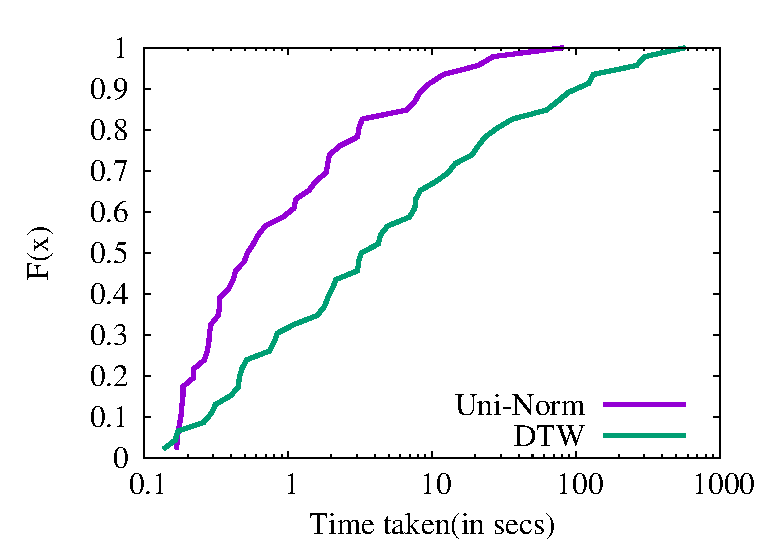
\includegraphics[scale=0.5]{figs/time_cdf.eps}
\caption{Computation time comparison of DTW and Uniform Norm for a subset of users}
\label{fig:time_dtw_uni}  
\end{subfigure}
~
\begin{subfigure}[t]{.4\textwidth}
\centering   
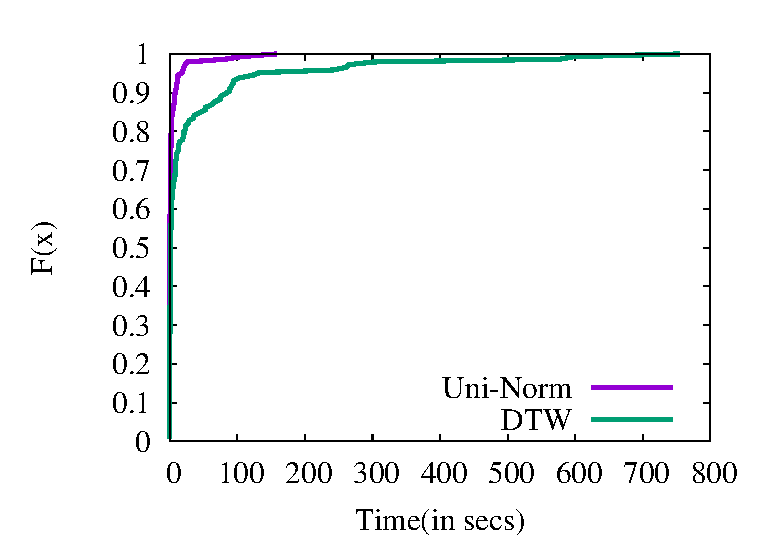
\includegraphics[scale=0.5]{figs/time_cdf_full.eps}
\caption{Computation time comparison of DTW and Uniform Norm for all the users}
\label{fig:time_dtw_full}  
\end{subfigure}
~
\begin{subfigure}[t]{.4\textwidth}
\centering   
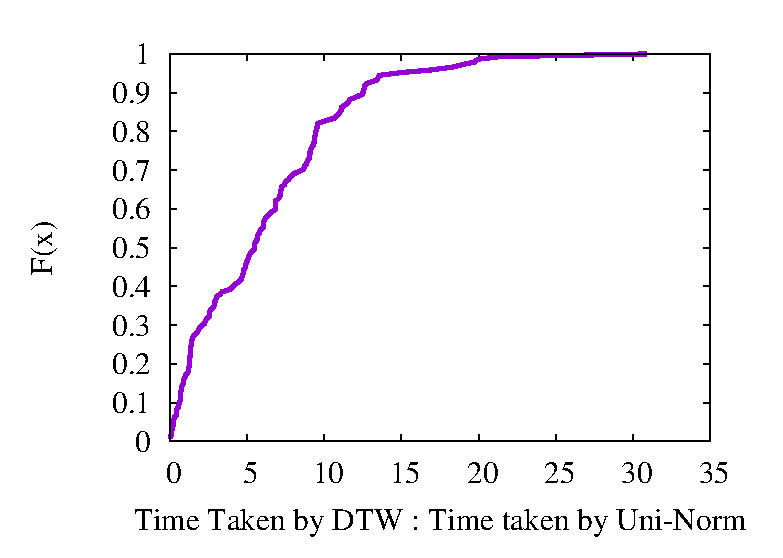
\includegraphics[scale=0.5]{figs/ratio_dtw_uni_cdf.eps}
\caption{CDF of the ratio of time taken by DTW to time taken by Uniform Norm}
\label{fig:time_dtw_ratio}  
\end{subfigure}
\caption{Computation Time Comparison between DTW and Uniform Norm}
\label{fig:time_dtw}
\end{figure*}
\end{comment}

\begin{figure}
	\centering     
	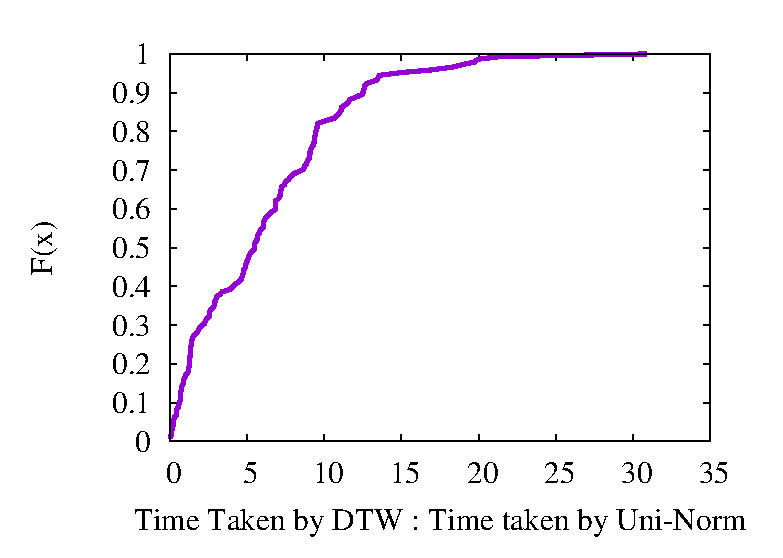
\includegraphics[scale=0.5]{figs/ratio_dtw_uni_cdf.eps}
	\caption{DTW vs. $\UN$: CDF of the speedup ratio}
	\label{fig:time_dtw_ratio}  
\end{figure}

We first compare different distance measures and discuss their effects. As discussed, DTW is a non-metric measure, and hence cannot be used in standard popular clustering algorithms to provide guaranteed optimal clusters. Moreover, the complexity of computing the distance-matrix between all trajectory pairs is exorbitant. Figure~\ref{fig:time_dtw_ratio} shows the CDF of the ratio of the time taken to compute the distance matrix for all users using DTW to that of $\UN$ metric. $\UN$ is a $5\times$ faster than DTW at the median. The larger the number of points in the trajectory the greater is the time to compute DTW. $\UN$ distance is invariant of number of samples since we consider the trajectory as a smooth curve and re-sample it for a constant number of times (100 equi-distant points in our case).


\subsection{Effectiveness of Summary Clusters}
\label{sec:evalSumm}
We first compare the effectiveness of DBSCAN, and then we evaluate different distance measures in hierarchical clustering. 

\paragraph{DBSCAN}
\label{sec:dbscanEval}
\begin{figure}
	\centering     
	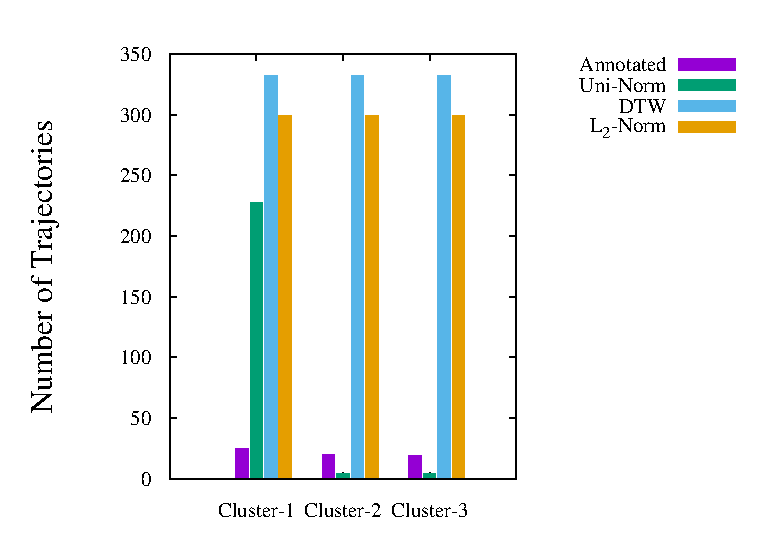
\includegraphics[scale=0.5]{figs/bar_dbscan.eps}
	\caption{DBSCAN with DTW, $\LP$ and $\UN$ distance measures: DBSCAN performs poorly on all evaluated distance measures}
	\label{fig:DBSCAN_bar}  
\end{figure}

Figure~\ref{fig:DBSCANRes} visually demonstrated that DBSCAN resulted in bad clusters using $\UN$ distance metric. Figure~\ref{fig:DBSCAN_bar} shows the effectiveness of DBSCAN under different distance measures (DTW, $\LP$ and $\UN$). 

For DBSCAN, we again use the recommended \text{Sorted $k$-Graph} methodology of finding the optimal input parameters with DTW and $\LP$. As shown in the Figure~\ref{fig:DBSCANRes}, DBSCAN aggregates too many trajectories. We conjecture that large cluster size is due to the large number of reachability paths that are found in the data-set. Most of the trajectories can be associatively reachable to large group of other trajectories, which will make it harder to cut the cluster containing only the similar trajectories. Moreover, even if the above problem is resolved, DBSCAN will be unable to segregate user's trajectories where there are a set of similar long trajectories and similar small trajectories (as explained in Section~\ref{sec:dbscan}).

\paragraph{Detailed Analysis of clustering techniques}
\label{sec:hierConfs}
\begin{figure*}
        \centering
        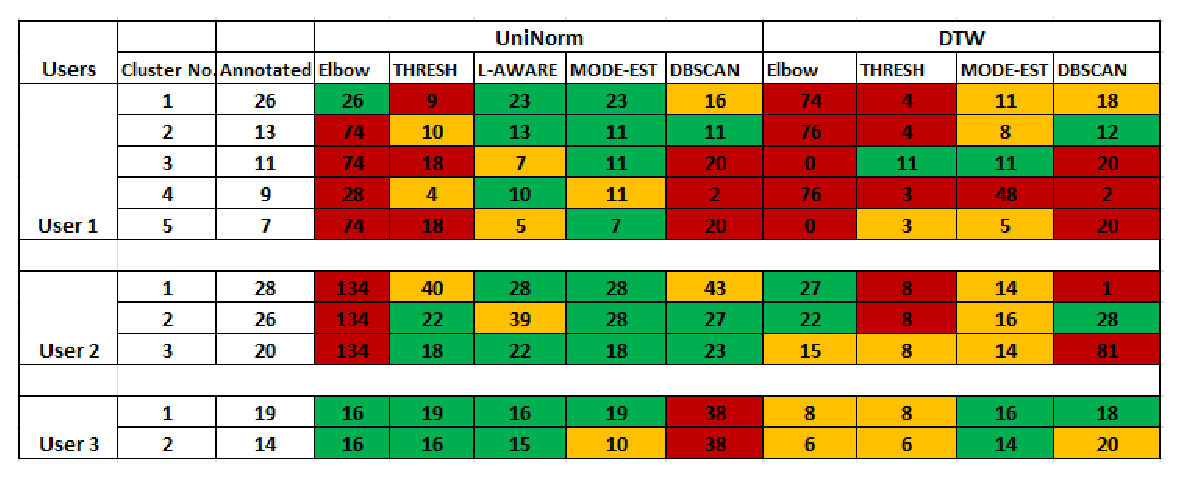
\includegraphics[scale=0.7]{figs/table.eps}
        \caption{Hierarchical clustering with different approaches: Green=$20$\% deviation from ground truth; Yellow=$\left[20-60\right]$\% deviation; Red= $> 60$ \% deviation}
        \label{fig:table}
 \end{figure*}

\begin{figure*}[t!]
    \centering
    \begin{subfigure}[t]{.3\textwidth}
        \centering
        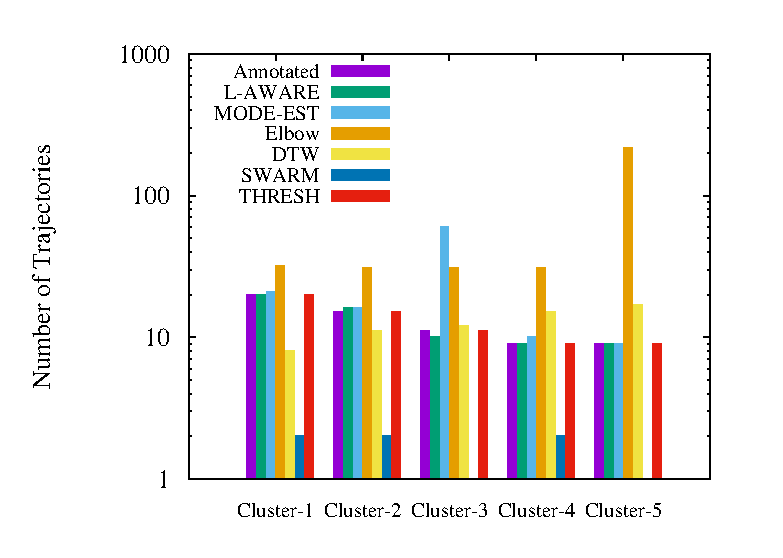
\includegraphics[scale=0.4,keepaspectratio]{figs/bar_user014.eps}
        \caption{User 4}
        \label{fig:user1}
    \end{subfigure}%
    ~
    \begin{subfigure}[t]{.3\textwidth}
        \centering
        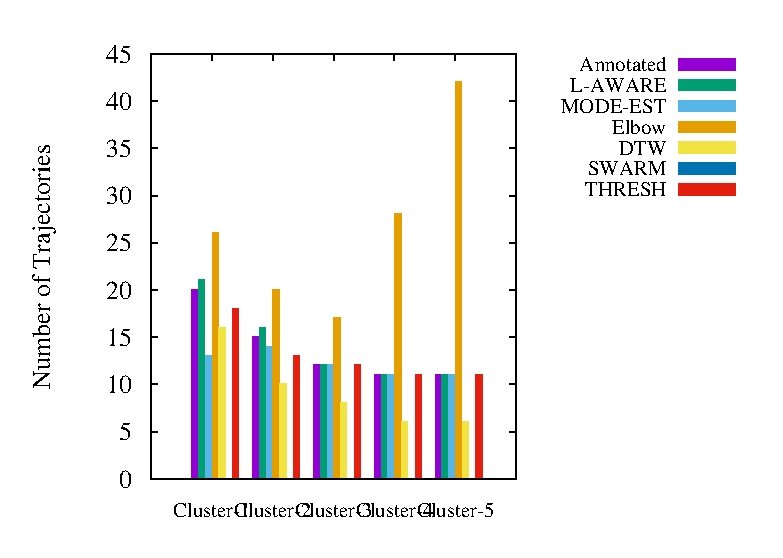
\includegraphics[scale=0.4,keepaspectratio]{figs/bar_user010.eps}
        \caption{User 5}
        \label{fig:user2}
    \end{subfigure}
   \caption{Cluster Effectiveness for $2$ random users: SWARM fails to report clusters for User-5, and reports poor clusters for User-4}
    \label{fig:bargrph}
\end{figure*}

We now compare different different type of distance metrics and cluster identification techniques. 
A single metric to judge the effectiveness of different user's multiple cluster summaries in various approaches is challenging. Existing simple metrics, such as Silhouette coefficient (which we will evaluate later), will not throw light various aspects of trajectory summarization such as the type of top clusters exposed and number of trajectories within the clusters. Hence, we randomly chose $5$ users, and hand-annotated the ``ground truth'' by visualizing their trajectories on the map using the tool we have developed (Section~\ref{sec:vis}). 

We evaluate various hierarchical clustering approaches and DBSCAN for the $3$ users. Table~\ref{fig:table} compares the top clusters predicted by different schemes for the four users. The rows indicate the user and the top-k cluster of each user. The columns describe each distance measure coupled with a particular clustering scheme. We have not included \lthAware metric for DTW since the trajectory length value (in km) and the standard deviation of pair-wise distance between trajectory predicted by DTW are not in the same units. The color coding indicates how far the ground truth and the predicted values are in each of the top clusters. 

Using the $\UN$ metric, we evaluate hierarchical clustering approaches to choose summary clusters using $4$ methods: Elbow method, \thresh, \lthAware, \modal. We also compare the effectiveness of DBSCAN. Hierarchical clustering with Elbow, which is one of the most popular algorithms to detect the right number of clusters, performs very poorly among all the schemes. DBSCAN is has a poor performance. The techniques proposed in this paper (\thresh, \lthAware, and \modal) perform progressively better for these users. Under the DTW distance measure, the results are similar there Elbow and DBSCAN performing poorly. 

Figure~\ref{fig:bargrph} exhaustively compares top-clusters for the other $2$ users, including SWARM technique. Here \lthAware and \modal performs the best, and SWARM performs poorly. In summary, it is clear that Hierarchical clustering with \modal and \lthAware cluster identification method provides superior summary clusters.

\paragraph{Overall clustering effectiveness}
\begin{figure*}
\centering     
\begin{subfigure}[t]{.32\textwidth}
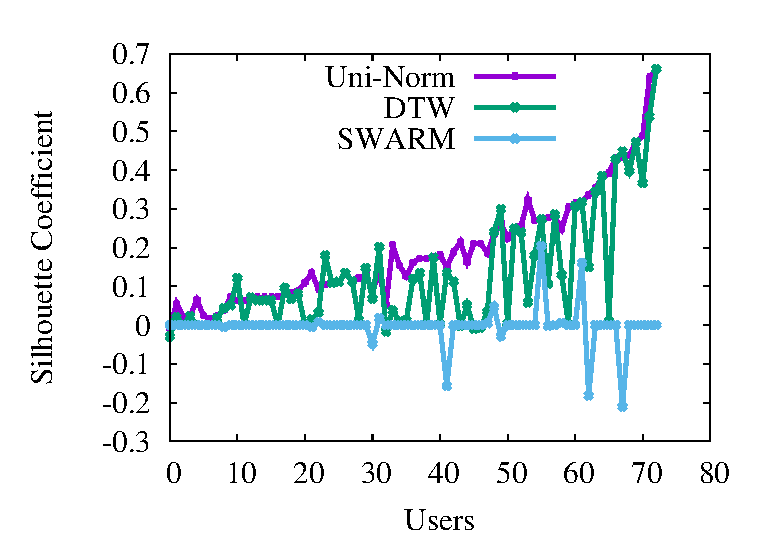
\includegraphics[scale=0.4]{figs/silFinal.eps}
\caption{User-specific Silhouette values for popular clustering schemes}
\label{fig:SWARM_OD}  
\end{subfigure}
~
\begin{subfigure}[t]{.32\textwidth}
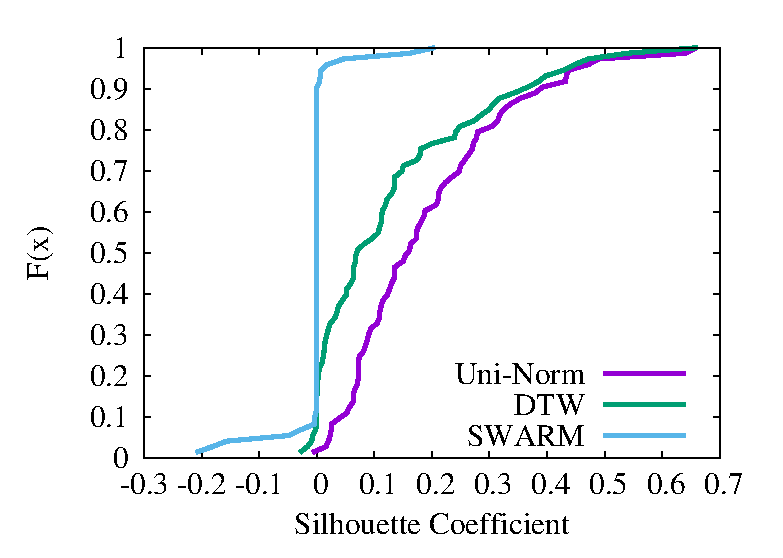
\includegraphics[scale=0.4]{figs/sil_cdfFinal.eps}
\caption{CDF of Silhouette Values}
\label{fig:cdf_sil}  
\end{subfigure}
~
\begin{subfigure}[t]{.32\textwidth}
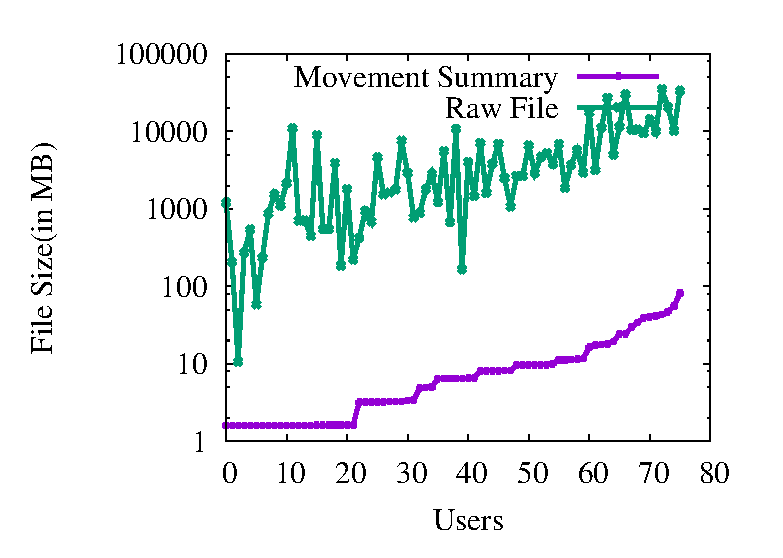
\includegraphics[scale=0.4]{figs/size_line.eps}
\caption{Storage compression: Storing only summary trajectories saves orders of magnitude space}
\label{fig:size_line}  
\end{subfigure}
\label{fig:sil}  
\end{figure*}

As discussed in the previous paragraph, a single metric that scores the clustering effectiveness for a particular application is hard to derive. A detailed comparison shown in Figure~\ref{fig:table} highlights the effectiveness of summaries for individual users. We now compare the effectiveness of the main clustering schemes for all the users in the data-set. 

Silhouette Coefficient(SC) is a widely used function for finding the clustering effectiveness. SC is based on the cohesion and the separation of clusters formed. The cohesion ( $a(x)$ )  is defined as the average distance of $x$ to all other vectors in the same cluster. The separation ($b(x)$) is defined as the minimum of the average distances of $x$ to the vectors in other clusters.

The silhouette coefficient $s(x)$ of a data point $x$ is then defined as 
\begin{equation}
s(x)=\frac{b(x)-a(x)}{max(a(x),b(x))}.
\end{equation}

The Silhouette Coefficient (SC) of the data-set is the average over all the points given by
\begin{equation}
\operatorname{SC}=\frac{1}{N}\sum_{i=1}^{N}s(x).
\end{equation}
\noindent SC is between [-1,1], where values closer to 1 representing better formed clusters. 

Figure~\ref{fig:SWARM_OD} compares the SC values for Hierarchical clustering using $\UN$ (Uni-Norm) and DTW (DTW) distance measures, where optimal clusters are selected by \modal technique. It also compares with SWARM approach of trajectory clustering. Figure~\ref{fig:SWARM_OD} shows that $\UN$ and DTW outperform SWARM for all the users. 

Figure~\ref{fig:cdf_sil} shows the CDF plot of the SC values. $\UN$ outperforms DTW by around 0.1 SC value at median. Both the schemes show an enormous improvement over existing trajectory clustering mechanisms such as Swarm.

\subsection{Trip Compaction}
We now show the benefits of storing summary trajectories instead of the entire raw trajectories. For this data-set, Fig \ref{fig:size_line} shows that there around $1-2$ orders of magnitude improvement in storing summaries over raw trajectories.
%\begin{figure*}
%\centering 
%\begin{subfigure}{0.5\textwidth} 
%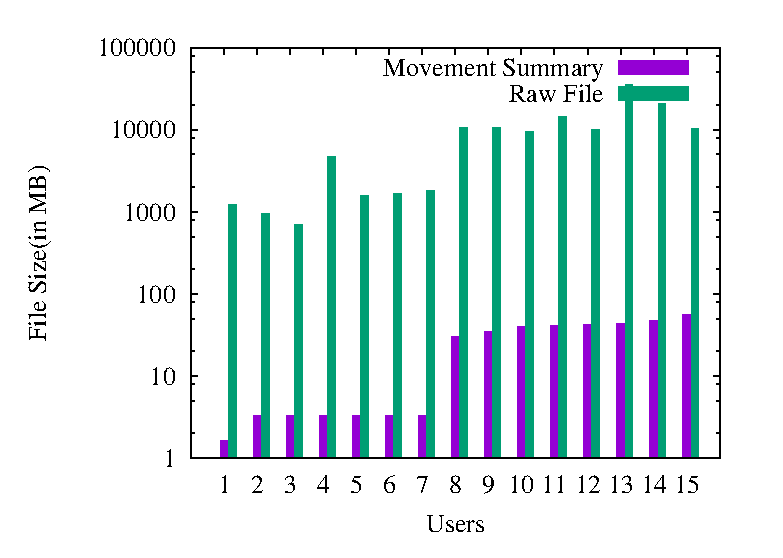
\includegraphics[scale=0.6]{figs/size_bar.eps}
%\caption{Comparisons of sizes for various users }
%\label{fig:size_bar}  
%\end{subfigure}

\begin{comment}
\begin{figure}
\centering    
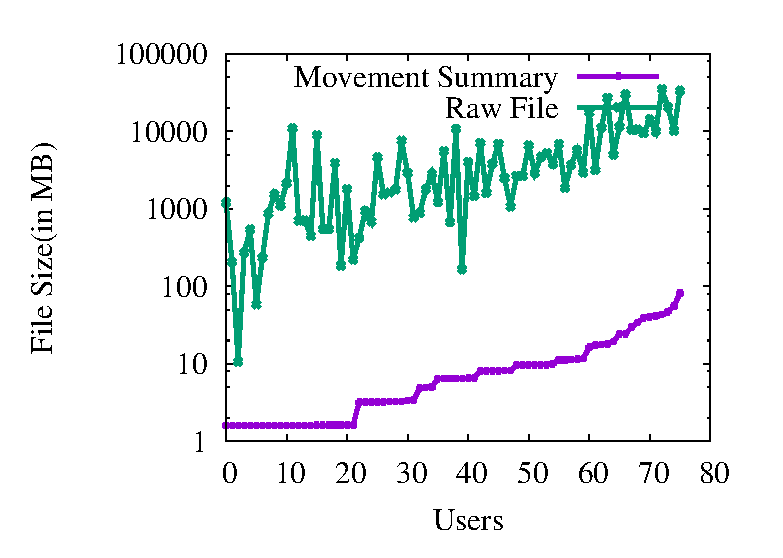
\includegraphics[scale=0.5]{figs/size_line.eps}
\caption{Difference in sizes over all the users}
\label{fig:size_line}  
\end{figure}
\end{comment}